\documentclass[10pt]{article}
\usepackage[a4paper, 
 	width = 150mm,
 	height = 250mm]{geometry}
\usepackage{fontspec}
	\setmonofont{Inconsolata}
	\setlength{\parskip}{0.25em}
	\setlength{\parindent}{0pt}
\usepackage{microtype}
\usepackage{color}
	\newcommand\greybox[1]{%
		\vskip\baselineskip%
		\par\hspace{18pt}\colorbox{lightgray}{%
			\begin{minipage}{\textwidth-36pt}#1\end{minipage}%
		}%
		\vskip\baselineskip%
	}
\usepackage{booktabs}
\usepackage{amssymb}
\usepackage{enumitem}
\usepackage{graphicx}
\usepackage{minted}
\usepackage{tcolorbox}
	\tcbuselibrary{minted,skins}
	\newtcblisting{bashcode}{
		listing engine=minted,
		colback=lightgray,
		colframe=white,
		listing only,
%		minted style=colorful,
		minted language=bash,
%		minted options={linenos=true,texcl=true},
		left=1mm,
	}
\newtcblisting{pycode}{
	listing engine=minted,
	colback=lightgray,
	colframe=white,
	listing only,
	%		minted style=colorful,
	minted language=python,
	%		minted options={linenos=true,texcl=true},
	left=1mm,
}
	\definecolor{SU}{RGB}{0, 46, 95}
	\definecolor{lightgray}{RGB}{245, 245, 245}
\usepackage{hyperref}
\hypersetup{
 	colorlinks,
 	citecolor = black,
 	filecolor = black,
 	linkcolor = SU,
 	urlcolor = SU,
 	pdfauthor = {Leonard Blaschek},
 	pdftitle = {phenotyping guide},
 	pdfkeywords = {Lignin methods}
}
 
\title{Guidelines for image based phenotyping of \textit{A. thaliana}}
 
\author{Leonard Blaschek}
 
\begin{document}
\maketitle

\section*{Why we do image based phenotyping}

We perform image based automated phenotyping to measure more parameters of plant growth at a higher temporal resolution than we could feasibly do using manual methods. Not only do image based approaches allow us to measure plants' height, area, colour and overall shape throughout their life cycle, the high quality images themselves can be used to measure additional features or phenotypes later on. As with all image analysis approaches, the quality of the input images is the single most important variable in determining success. In the approach implemented by me, two imaging setups are used, depending on the developmental stage of the \textit{A. thaliana} plants. In this document, I will try to summarise what you need to know about image acquisition, automated phenotyping and data analysis.

\tableofcontents


\section{Image acquisition}

\subsection{Rosette growth}

From germination until bolting, the plants are best imaged from the top. One big advantage of this is that the pots can be left in the tray, meaning that 15 plants can be analysed from a single picture. As you can see from the example image in figure \ref{fig:top}, I acquire the images without labels. Instead, I have labels on the side of the pots (see figure \ref{fig:front_before}). That of course means that you have to be very careful to document the order of pots (genotypes/replicates) in each tray, and orient the trays in the same way in each picture (put a label on one side of the tray to make sure you do not accidentally flip it 180°). You also need to carefully document which picture shows which tray. Lastly, bright markers (any colour that stands out, I use light blue) on the outer edges of the tray allow you to easily crop the image to the area of interest in the analysis. Lastly, taking the pictures always in the same order will save you a lot of time in the analysis (see section \ref{prep}).
	
\begin{figure}[!h]
	\centering
	\includegraphics[height=0.3\textheight]{21_1}
	\caption[Example image of a top-view image.]{\textit{A. thaliana} plants during their vegetative phase (before bolting of the inflorescence stem), imaged from the top. The image should cover the whole tray and the colour card to the left, both of which should be oriented in parallel with the image borders. Acquisition parameters need to be chosen to avoid over-exposure. Also note the blue stickers on the corners of the tray, which are later used to define the area of interest for the image analysis.}
	\label{fig:top}
\end{figure}

\noindent In order to avoid over-exposure, the following acquisition parameters have proven successful in our setup:

\begin{itemize}
	\item 50 mm objective
	\item 1/125 s exposure time
	\item f5.6 aperture
	\item 800 ISO sensitivity
	\item white balance set to "Incandescent"
\end{itemize}

\subsection{Inflorescence growth}

After the plants bolt, we switch to imaging from the front. Now we have to image each plant individually. Make sure that the label on the front of the pot is clearly visible in each image. Everything in the image that is \textit{not} the plant or the colour card, such as labels, sticks, pots, \textit{etc.} should be of a colour that is easy to distinguish from the plant. Because \textit{A. thaliana} can be green (leaves), white (flowers), purple (stressed leaves), yellow/beige/brown (plants in senescence), the ideal colour for foreign objects is blue (see stick in figure \ref{fig:front_after}). Just as with the rosette images, taking the pictures always in the same order will save you a lot of time in the analysis (see section \ref{prep}).

\begin{figure}[!h]
	\centering
	\includegraphics[height=0.3\textheight]{20201008_8}
	\caption[Example image of a front-view image.]{An \textit{A. thaliana} plant during its reproductive phase (after bolting of the influorescence stem, but \textbf{before} binding the stems to a stick), imaged from the front. The image should cover the whole plant and the colour card to the left, both of which should be oriented in parallel with the image borders. Acquisition parameters need to be chosen to avoid over-exposure. Also note the red label on the front of the pot, used for identification. This label can contain any amount of text, but should be blue or red, to avoid colour similarity to the plant itself.}
	\label{fig:front_before}
\end{figure}

\noindent For this stage, the following acquisition parameters have proven successful in our setup:

\begin{itemize}
	\item 50 mm objective
	\item 1/30 s exposure time
	\item f13 aperture
	\item 2000 ISO sensitivity
	\item white balance set to "Incandescent"
\end{itemize}

\subsection{Checklist for optimal images}

If you read through the above section, you should have a pretty good idea why we set up the pictures the way we do. Here is a little checklist to go through when you start taking images, to make sure you don't forget an important detail:

\begin{itemize}[label=$\square$]
\item \textbf{Correct perspective}: the camera should be oriented orthogonally to the sample, not angled up- or downwards; this avoids size distortions (if the trays look trapezoid instead of rectangular on the images, you're doing it wrong)
\item \textbf{Clean image area}: make sure that there is nothing unnecessary in the image and clean the black background from debris
\item \textbf{Distinct colour for foreign objects:} whatever remains in the image that \textit{is not} the plant itself should have a colour that is distinct from any part of the plant, ideally blue
\item \textbf{Avoid obstruction:} labels, sticks and the colour card should be arranged in a way that does not obscure any part of the plant; for tray images remove pot labels completely, for images of bolted plants place the labels in front of the pot and move the stick behind the shoots
\end{itemize}

\begin{figure}[!h]
	\centering
	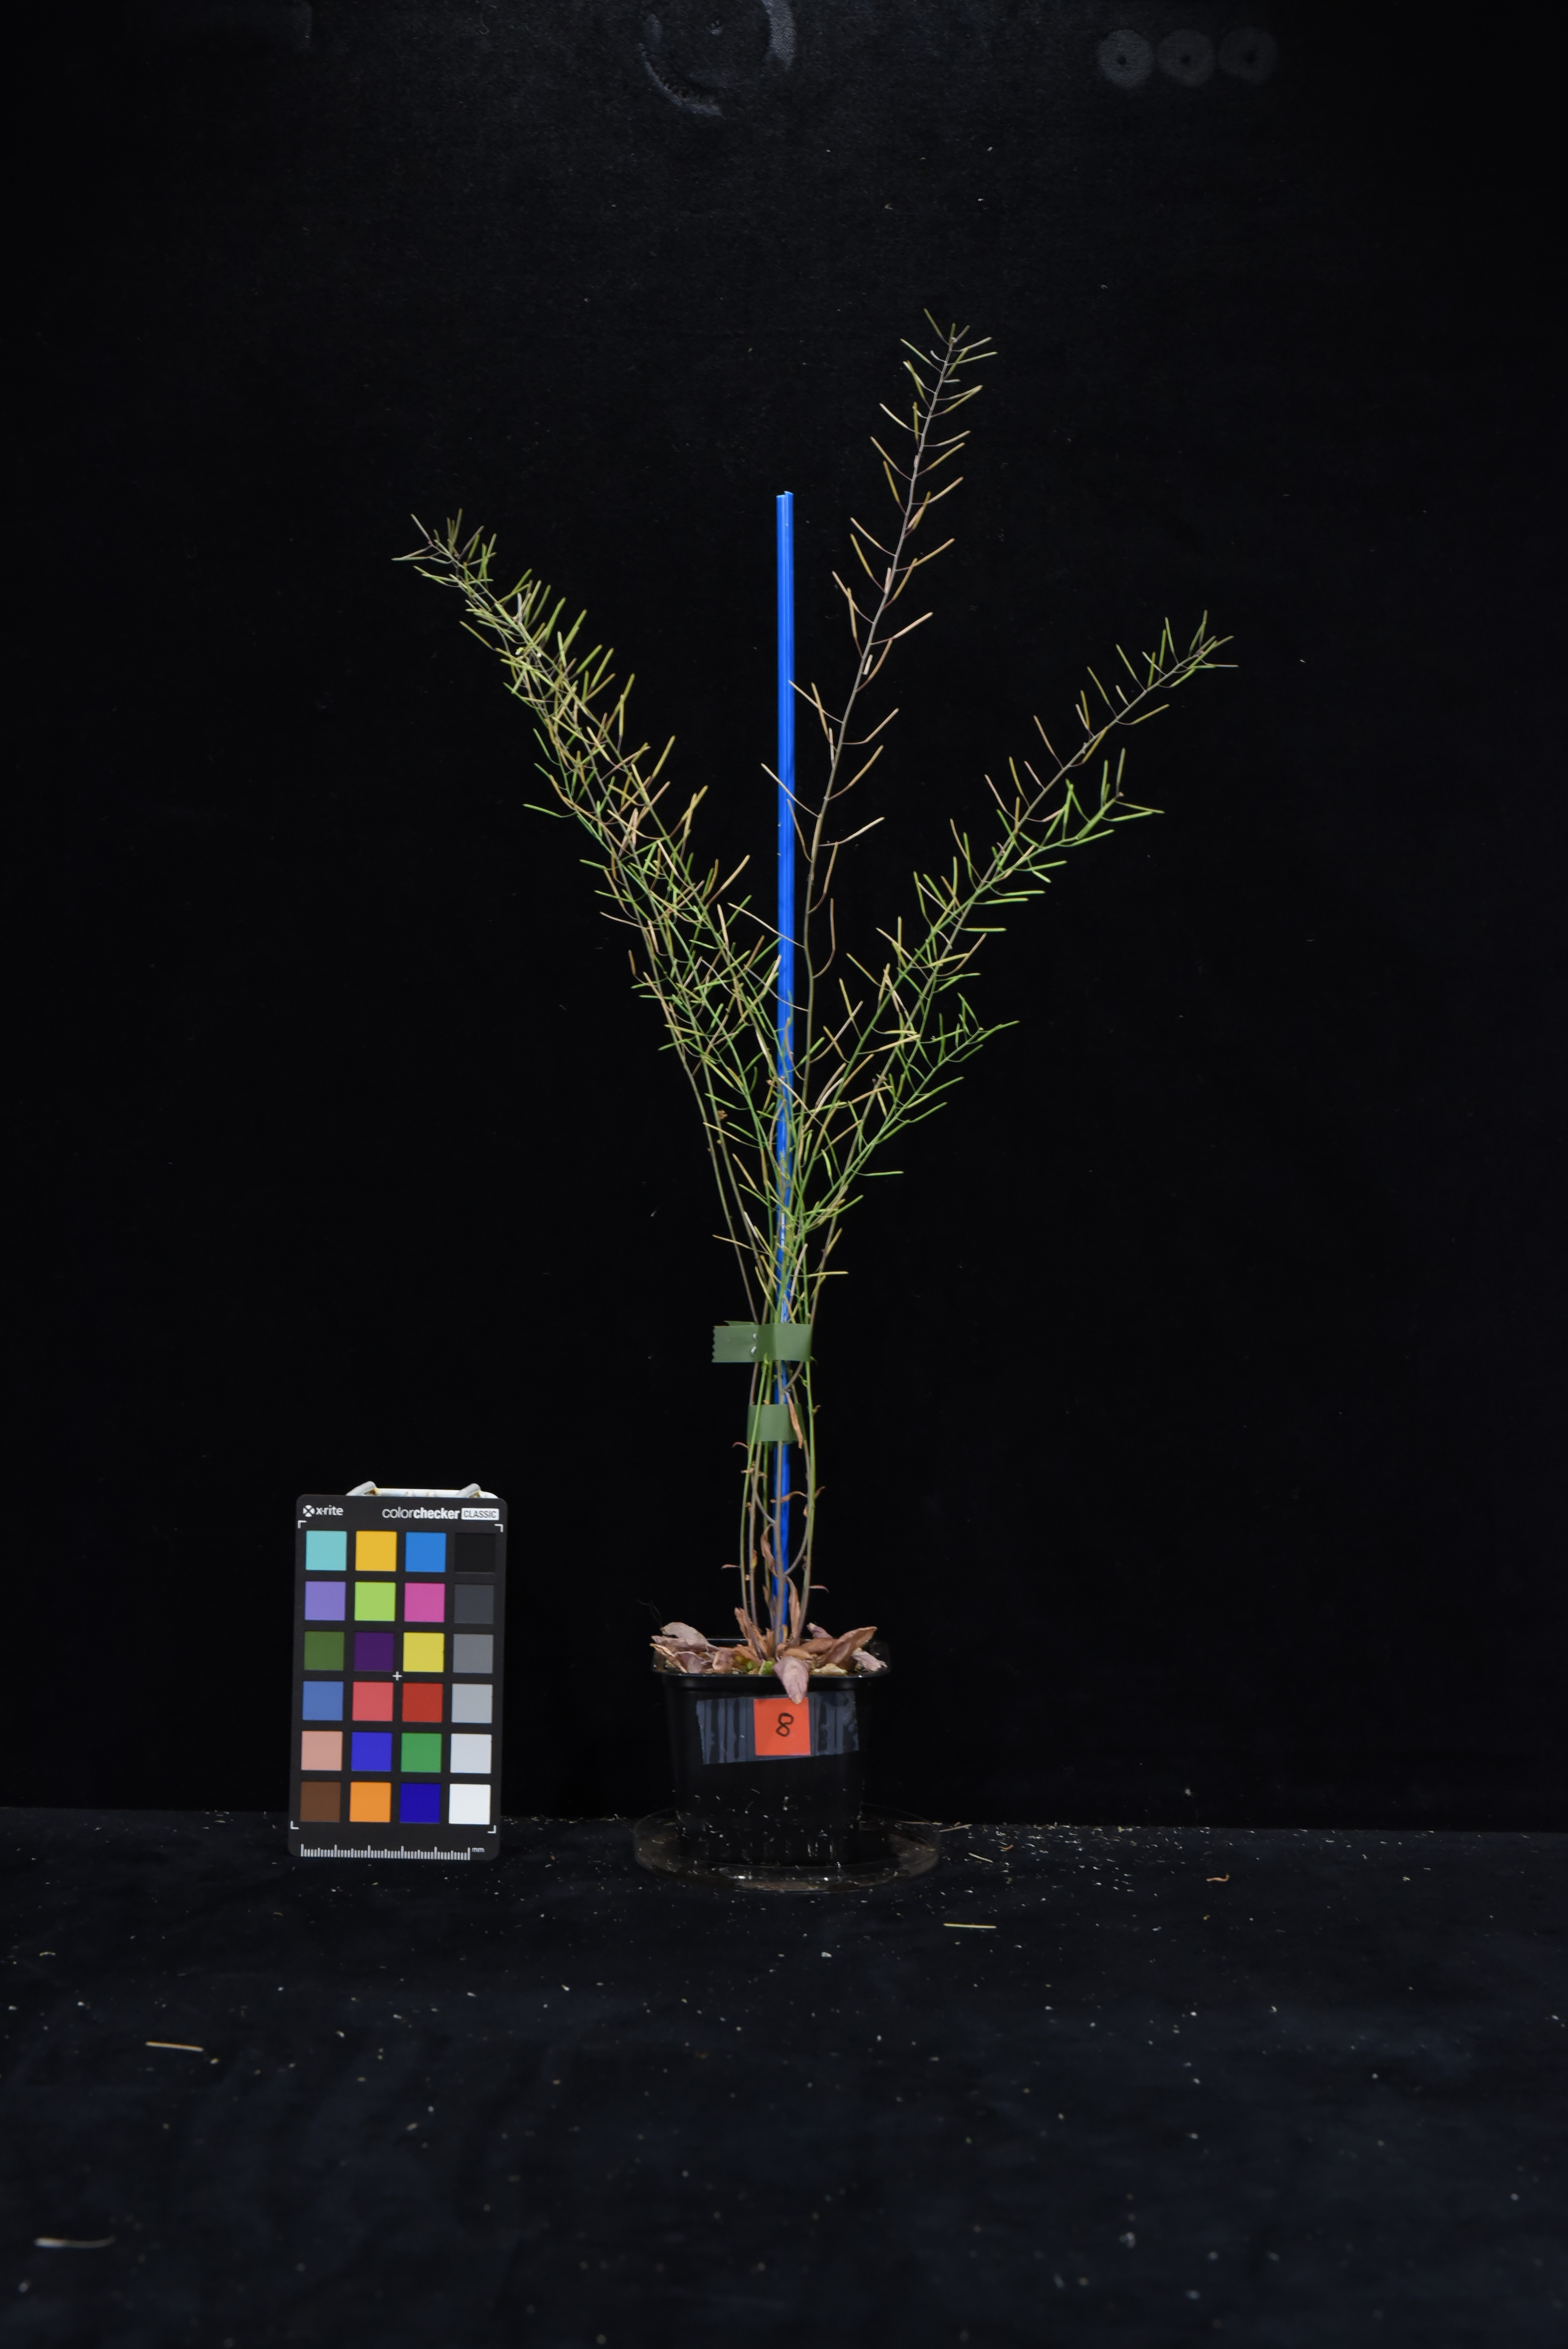
\includegraphics[height=0.3\textheight]{20201029_8}
	\caption[Example image of a front-view image.]{An \textit{A. thaliana} plant during its reproductive phase (\textbf{after} binding the stems to a stick), imaged from the front. Just like the label, the stick should ideally be blue to facilitate separation from the plant itself in the analysis.}
	\label{fig:front_after}
\end{figure}

\section{Image metadata\label{prep}}

If we want to automate the image analysis, we need to make sure that each image contains all the metadata we need to assign the output to the correct plant. Imagine for example we take an image of a tray with 15 pots from the top and save that image as \texttt{DSC\_2487.JPG}. If we input this image into the analysis pipeline, it will output results for each of the 15 plants on the tray, which it will call \texttt{DSC\_2487.JPG\_1, DSC\_2487.JPG\_2} and so on. But what genotype is plant \texttt{DSC\_2487.JPG\_1} and how old was the plant when the picture was taken? The easiest way to embed metadata in your image is in the image name. If we for example rename our image \texttt{DSC\_2487.JPG} to \texttt{13\_2.JPG}, we have the day past germination (13) and the tray number (2) right in the file name. 

You can rename the pictures by hand, but if you have followed my advice above and took the pictures always in the same order, we can also automate the renaming. The following script works on MacOS and Linux, and renames all \texttt{.JPG} files in the same folder. So create one folder with the picture from the top and one folder with the pictures from the front. The script renames the images with the day past germination and the number of each tray or plant. For example, if your plants germinated roughly on the 24th of July 2020, you'd set \texttt{germination=20200824}. If you have three full trays of plants, you would set the \texttt{end=3}  for the pictures taken from above, and \texttt{end=45} for the pictures of the individual plants taken from the front.
 
\begin{bashcode}
	#!/bin/bash
	# define the date of germination for DPG (days past germination) calculation
	germination="20200824"
	# number of the first sequentially numbered trays/plants
	start=1
	# number of the last sequentially numbered trays/plants
	end=3
	# rename images by DPG and tray/plant number
	a=$start
	for i in *.JPG; do
		var1="_"
		DPG=$(( ($(date -r "$i" +%s) - $(date --date=$germination +%s) )/(60*60*24) ))
		mv -i -- "$i" "$DPG$var1$a.jpg"
		if [ "$a" -lt $end ]
		then
			let a=a+1
		else
			let a=$start
		fi
	done
\end{bashcode} 


\section{Image exploration in Fiji}

To get a feeling for the images, open one of them in \href{https://imagej.net/Fiji/Downloads}{Fiji} and explore how you can segment and measure different parts of the plant. A very useful function for this is \texttt{Image} $\rightarrow$ \texttt{Adjust} $\rightarrow$ \texttt{Color Threshold...} (use the LAB colour space). To calibrate any height or area measurements, you can define the pixel size using the ruler on the bottom of the colour card.

\section{High-throughput analysis in Python and PlantCV}

You can do the complete analysis in Fiji, but depending on the amount of images you have, this might be prohibitively time consuming. The alternative is a programmatic approach that automates same principles of image analysis that we would use in Fiji. \href{https://plantcv.danforthcenter.org/}{PlantCV} is a Python library that was specifically designed for plant phenotyping. Getting started with it is more complicated than using Fiji, but once it is set up the reward is a highly reproducible analysis pipeline that needs minimal manual intervention. In the following I will outline the initial steps of working with our images in PlantCV. Beyond this short tutorial, I highly recommend the excellent official \href{https://plantcv.readthedocs.io/en/stable/}{documentation} of PlantCV. Lastly, if you are already familiar with PlantCV and want to skip ahead to the analysis pipeline optimised for our imaging setup, head over to my \href{https://github.com/leonardblaschek/plantcv}{Github page}.

\subsection{Installation}

Ideally, you are performing this analysis on the computer in the GMO room, on which Python and PlantCV are already set up. If not, the following steps will install the necessary software on your machine.

\paragraph{Install Anaconda}
\texttt{Anaconda} and its slimmed down version \texttt{Miniconda} are package and environment managers for Python. It allows you to create virtual environments for specific tasks, which simplifies work in Python immensely. If you do not have it installed already, I recommend \href{https://docs.conda.io/en/latest/miniconda.html}{\texttt{Miniconda}}. Simply follow the installation instruction for you operating system. If you are unsure, your operating system is almost definitely the 64-bit variant.

\paragraph{Install PlantCV}
If you are on Windows, start the \texttt{Anaconda Prompt}, on MacOS and Linux simply open a terminal window. To test that conda is properly installed, type:
  
\begin{bashcode}
	conda --version
\end{bashcode}

The prompt should then output the installed conda version, for example \texttt{conda 4.9.2}. If this worked as expected, we next need to add the channel containing the PlantCV package to the conda configuration:

\begin{bashcode}
	conda config --add channels conda-forge
\end{bashcode}

Now we install PlantCV in a new environment called \texttt{plantcv}:

\begin{bashcode}
	conda create -n plantcv plantcv
\end{bashcode}

Last we will activate our new environment and install some additional packages:

\begin{bashcode}
	conda activate plantcv # activate the plantcv conda environment
	conda install -c conda-forge jupyterlab # install JupyterLab
	conda install -c conda-forge imutils # install imutils
\end{bashcode}

\subsection{Optimisation in JupyterLab\label{opt}}

To see how well my (or any other) image analysis pipeline works for your specific images, first try it out on single images in \texttt{JupyterLab}. The advantage of this approach is that you get intermediate outputs at every step of the pipeline, easily letting you pinpoint any sections that need adjustment. First, make sure you are in the correct conda environment, then start up \texttt{JupyterLab}:

\begin{bashcode}
	conda activate plantcv # make sure you are in the correct conda environment
	jupyter-lab # start JupyterLab
\end{bashcode}

\texttt{JupyterLab} will start in your default browser, check for a newly opened tab if you already had a browser window open.

\subsubsection{Rosette growth}

Lets start with the images from the top. Download the \texttt{JupyterLab} file \href{https://github.com/leonardblaschek/plantcv/blob/master/tray_vis_allow_gaps.ipynb}{tray\_vis\_allow\_gaps.ipynb}, save it somewhere convenient (I would advise creating a dedicated \texttt{PlantCV} folder), and open it in JupyterLab. As you see, the code is split up in individual cells that can be run one at a time. 

\paragraph*{Cell 1} The first cell loads all necessary packages and defines that the intermediate output is directly printed into the JupyterLab notebook.

\paragraph*{Cell 2} In the second chunk, you need to change the path in the \texttt{pcv.readimage} function so that it leads to a representative picture of your plants. I would choose a full tray at an intermediate growth stage. \textit{There are some parts that are commented out which relate to colour correction. Ignore those for now.}

\paragraph*{Cells 3--5} The next three chunks identify the colour card, write it's size to file as a scale reference, and crop out the colour card so it doesn't interfere with the downstream analysis. \textit{Again, ignore the commented-out lines about colour correction.}

\paragraph*{Cell 6} Next, we identify the bright markers in the corners of the tray and crop the picture accordingly.

\paragraph*{Cell 7} This cell simply outputs the L, A and B channels of the LAB colourspace, and the H and S channels of the HSV colourspace (the V channel is roughly identical to the L channel of the LAB colourspace). The output purely serves to give you a better idea of which of these channels are suitable for segmentation. What makes a channel suitable for segmentation is the difference between the plant and the background. In most scenarios, the A and B channels will work best (figure \ref{fig:S_A}), but depending on your specific case, the others might be useful as well.

\begin{figure}[!h]
	\centering
	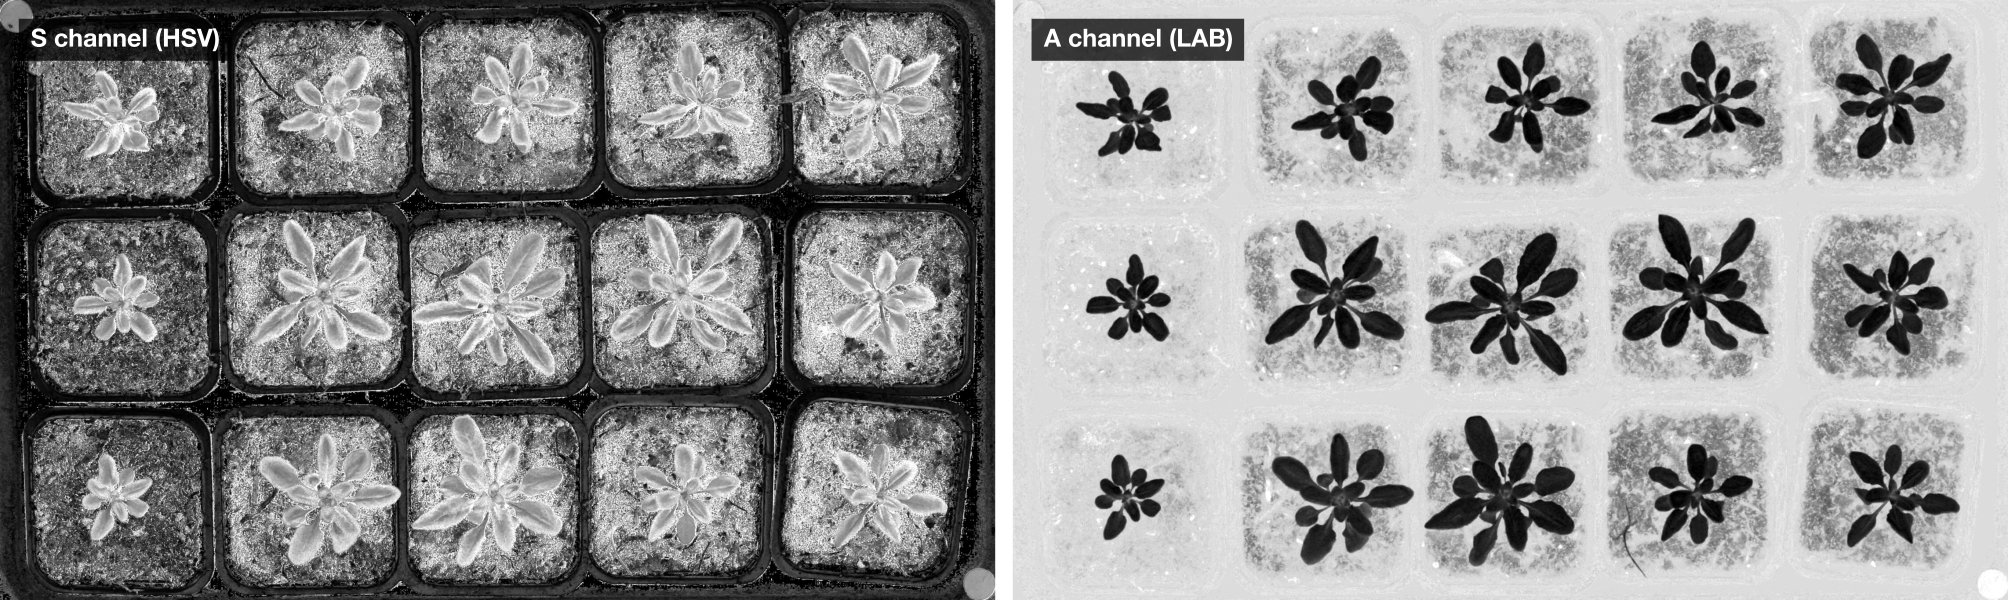
\includegraphics[width=0.95\linewidth]{S_A}
	\caption[S and A channels.]{The saturation (S) and red--green (A) channels from the HSV and LAB colourspaces respectively. The S channel is clearly not very useful in this example, while the clear difference between plant and background in the A channel makes the latter a prime candidate for image segmentation.}
	\label{fig:S_A}
\end{figure}

\paragraph*{Cell 8} This is the most important cell of the pipeline. Here, you use the channels identified in the previous cell to reliably segment the image so that only the plant remains, and the background is removed. In the file you downloaded, I use channels A, B, and H. For each of these, I create a threshold defining which pixels are classified as plant, and which as background. We then join these thresholds, only keeping the pixels that were classified as plant in all three channels.

After the thresholds have been applied, we filter and clean the image a little to remove any small incorrectly classified outliers. the \texttt{if--else} statement here relies on the consistent naming of your files, because it changes parameters depending on plant age. In early stages, we remove only very tiny outliers, because the plant itself is very small. In later growth stages, we can remove larger outliers without risking losing the plant.

\paragraph*{Cells 9--13} Here we cluster the pixels classified as plant into individual plants, and export one image for each plant. This is just so you have the segmented images for presentation purposes. If you took good pictures and chose the right thresholds in cell 8, the output of cell 12 should look like figure \ref{fig:clusters}.

\begin{figure}[!h]
	\centering
	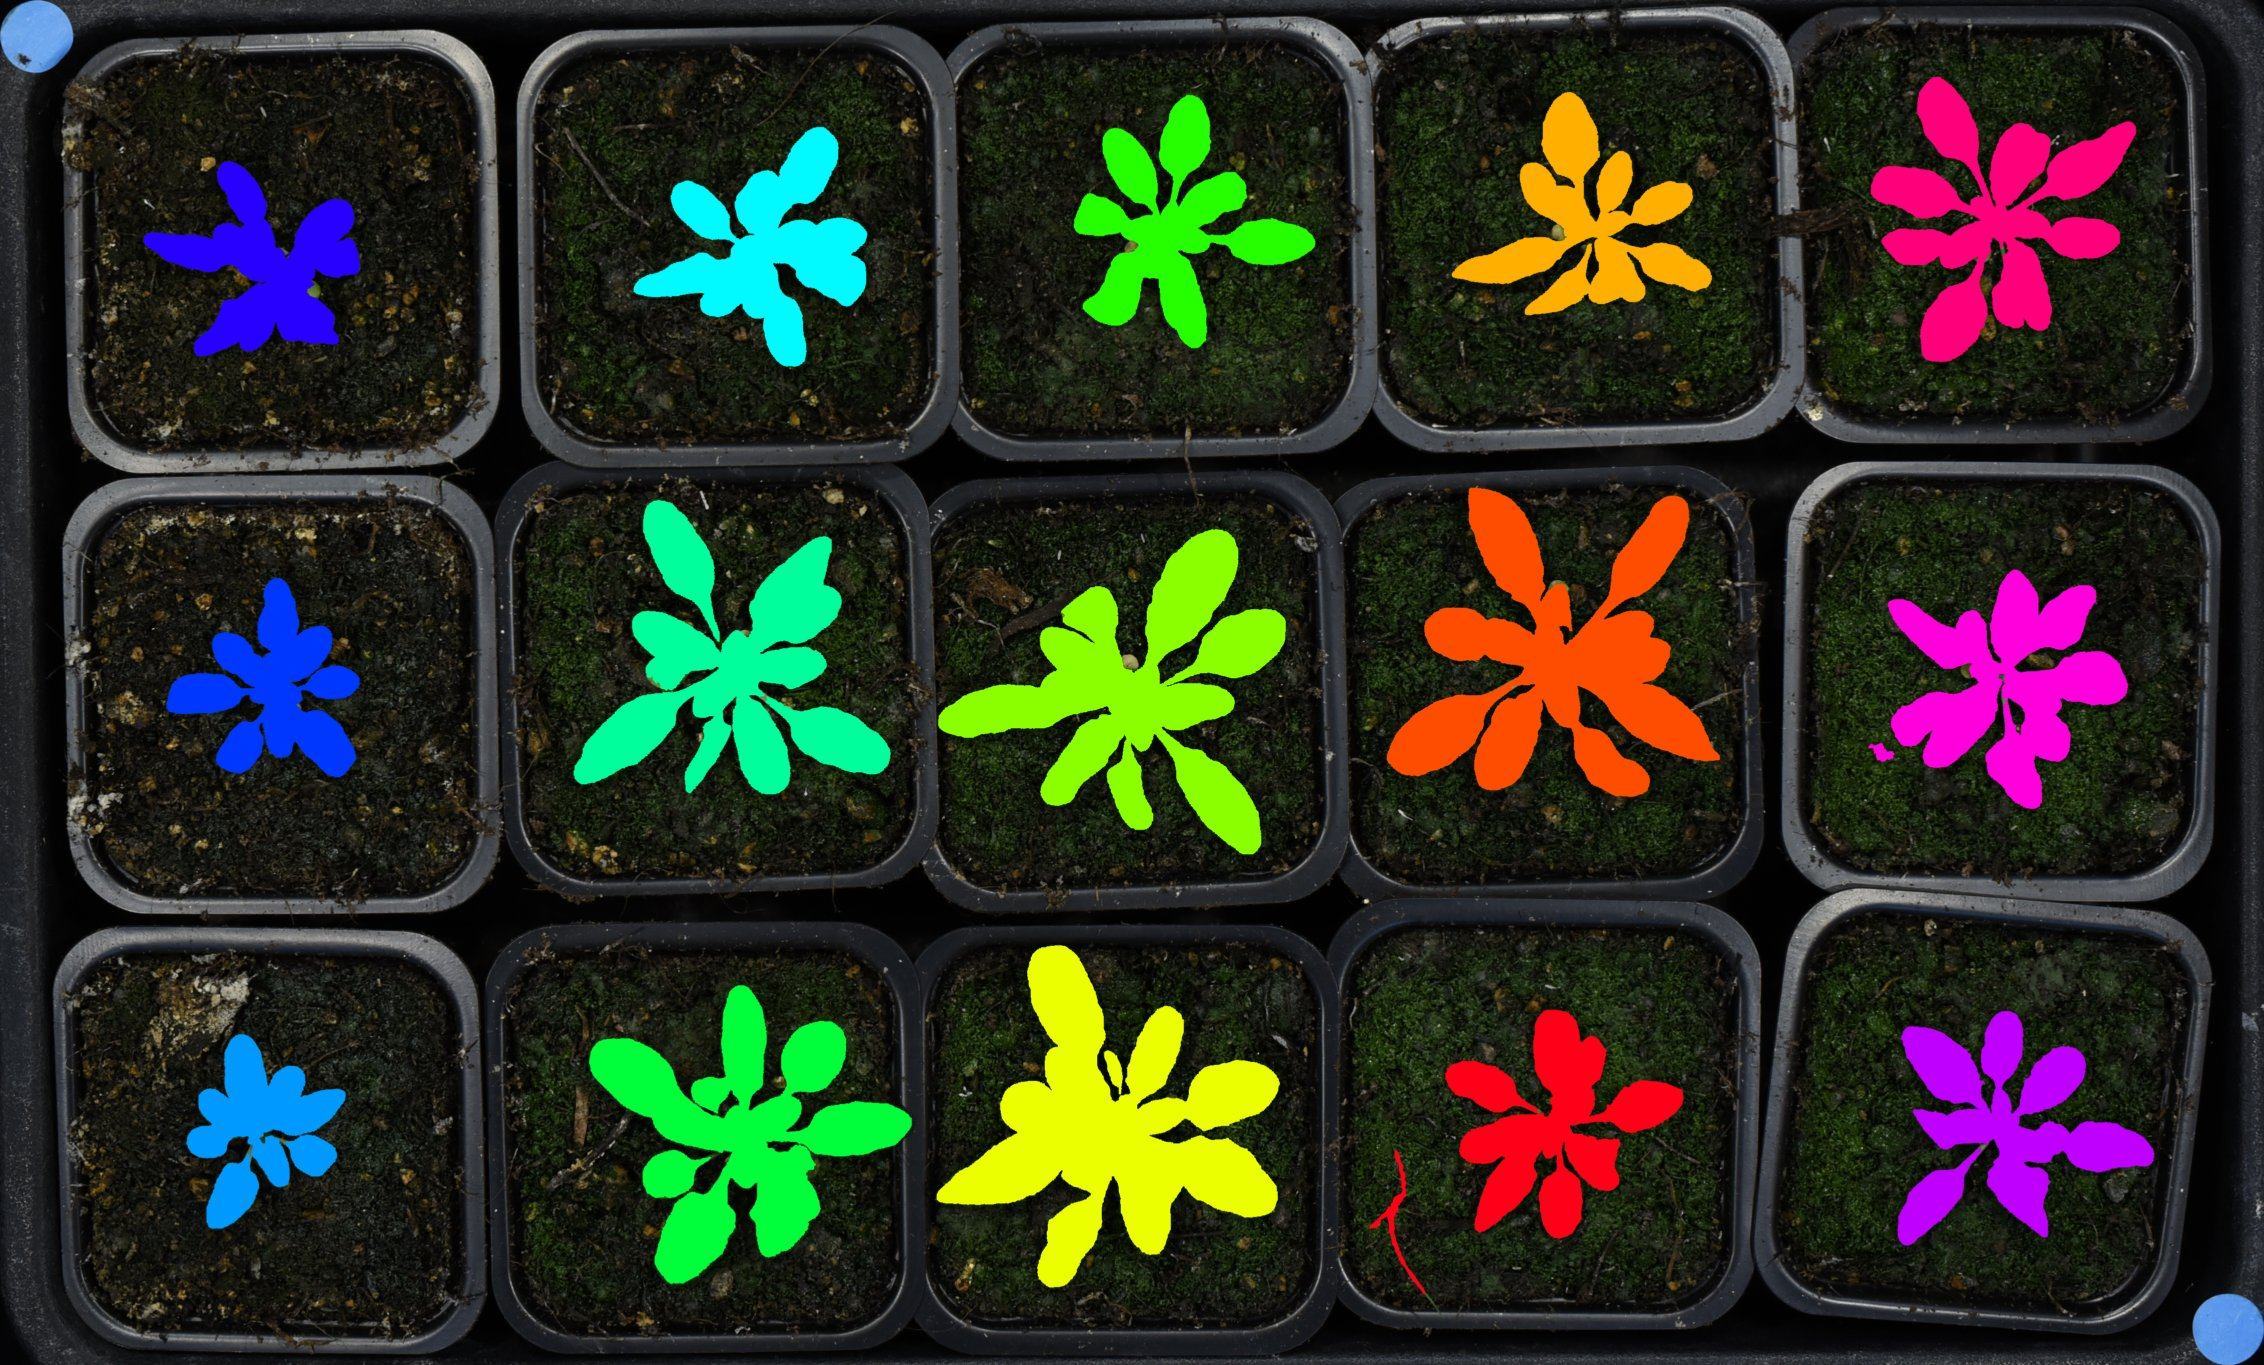
\includegraphics[width=0.6\linewidth]{clusters}
	\caption[Successfully clustered plants.]{Successful clustering of plant-pixels into individual plants. Note some minor miss-classifications like the string shaped contour in the red plant, which will be filtered out in the coming steps.}
	\label{fig:clusters}
\end{figure}

\paragraph*{Cell 14} This is the actual image analysis part. The function takes our segmented image, defines the regions-of-interest (ROIs) where it expects plants, and analyses each plant. It outputs parameters of rosette shape (area, compactness), colour (HSV), and morphology (leaf count) to \texttt{.json} files. The analysis also allows for holes, \textit{i.e.} trays with less than 15 pots or pots with no plants, without messing up your plant numbering.

\paragraph*{Final touches} Now the pipeline is optimised for the image you chose in the beginning. To make sure that it will work for your whole dataset, go through the JupyterLab notebook with other images, especially those from very early and very late stages. Adjust the thresholds in cell 8 to get the best results across your dataset. In early stages, too stringent thresholds will lead to the loss of leaves or whole plants, while the biggest problem in later stages is plant overlap. If two plants overlap, the pipeline will classify them as one plant, messing up your results. The only remedy for that is to open the respective images in any image manipulation software (Fiji/GIMP/Paint), and separating the plants by drawing black lines across their point of overlap.

\subsubsection{Inflorescence growth}

The pipeline for the inflorescence growth, \textit{i.e.} the pictures taken from the side, is very similar to the one for the rosette growth. Download the \href{https://github.com/leonardblaschek/plantcv/blob/master/plantcv_vis.ipynb}{plantcv\_vis.ipynb} file, and open it as described above. Below, I will highlight some parts that are different from the rosette pipeline or might need tweaking.

\paragraph*{Cell 3} At some point in later growth stages, you probably started tilting the camera by 90° to get the whole plant on the picture. In this cell, we detect whether the image was tilted to the left by checking the position of the colour card. If the image is tilted, we rotate it to the correct orientation and define a variable called \texttt{rotated} for use in coming cells. \textit{Note: if you tilted the camera to the right, we will need to think of another way to correct for that. Let me know.}

\paragraph*{Cell 6} This cell is equivalent to cell 8 in the rosette growth pipeline. The main difference is twofold. Firstly I also leverage the L channel here, because our background is uniformly black. Secondly, I define the hue threshold from two sides, a low and a high part. Combining these two thresholds with the \texttt{pcv.logical\_or()} function filters out only the blue, which is in the middle of the hue scale. Adjust the thresholds to fit your pictures.

\paragraph*{Cell 8} Here we define a static ROI. There are two sets of coordinates, depending on whether we rotated the picture previously or not. Only pixel clusters that are at least partly within this ROI will be used for analysis. The main use for this step is to filter out leaves, silliques and other debris that is on the ground. This means that the most important part of the ROI is its lower edge. The other thing to consider is that if you choose the ROI too small, imperfect segmentation can lead to parts of the plant being discarded when their connection to the rest of the plant is interrupted.

\paragraph*{Cell 11} This is the image analysis part. It outputs essentially the same data as you've seen for the rosette growth pipeline. If everything worked as it should, the output of this chunk should look like figure \ref{fig:inflorescence}.

\begin{figure}[!h]
	\centering
	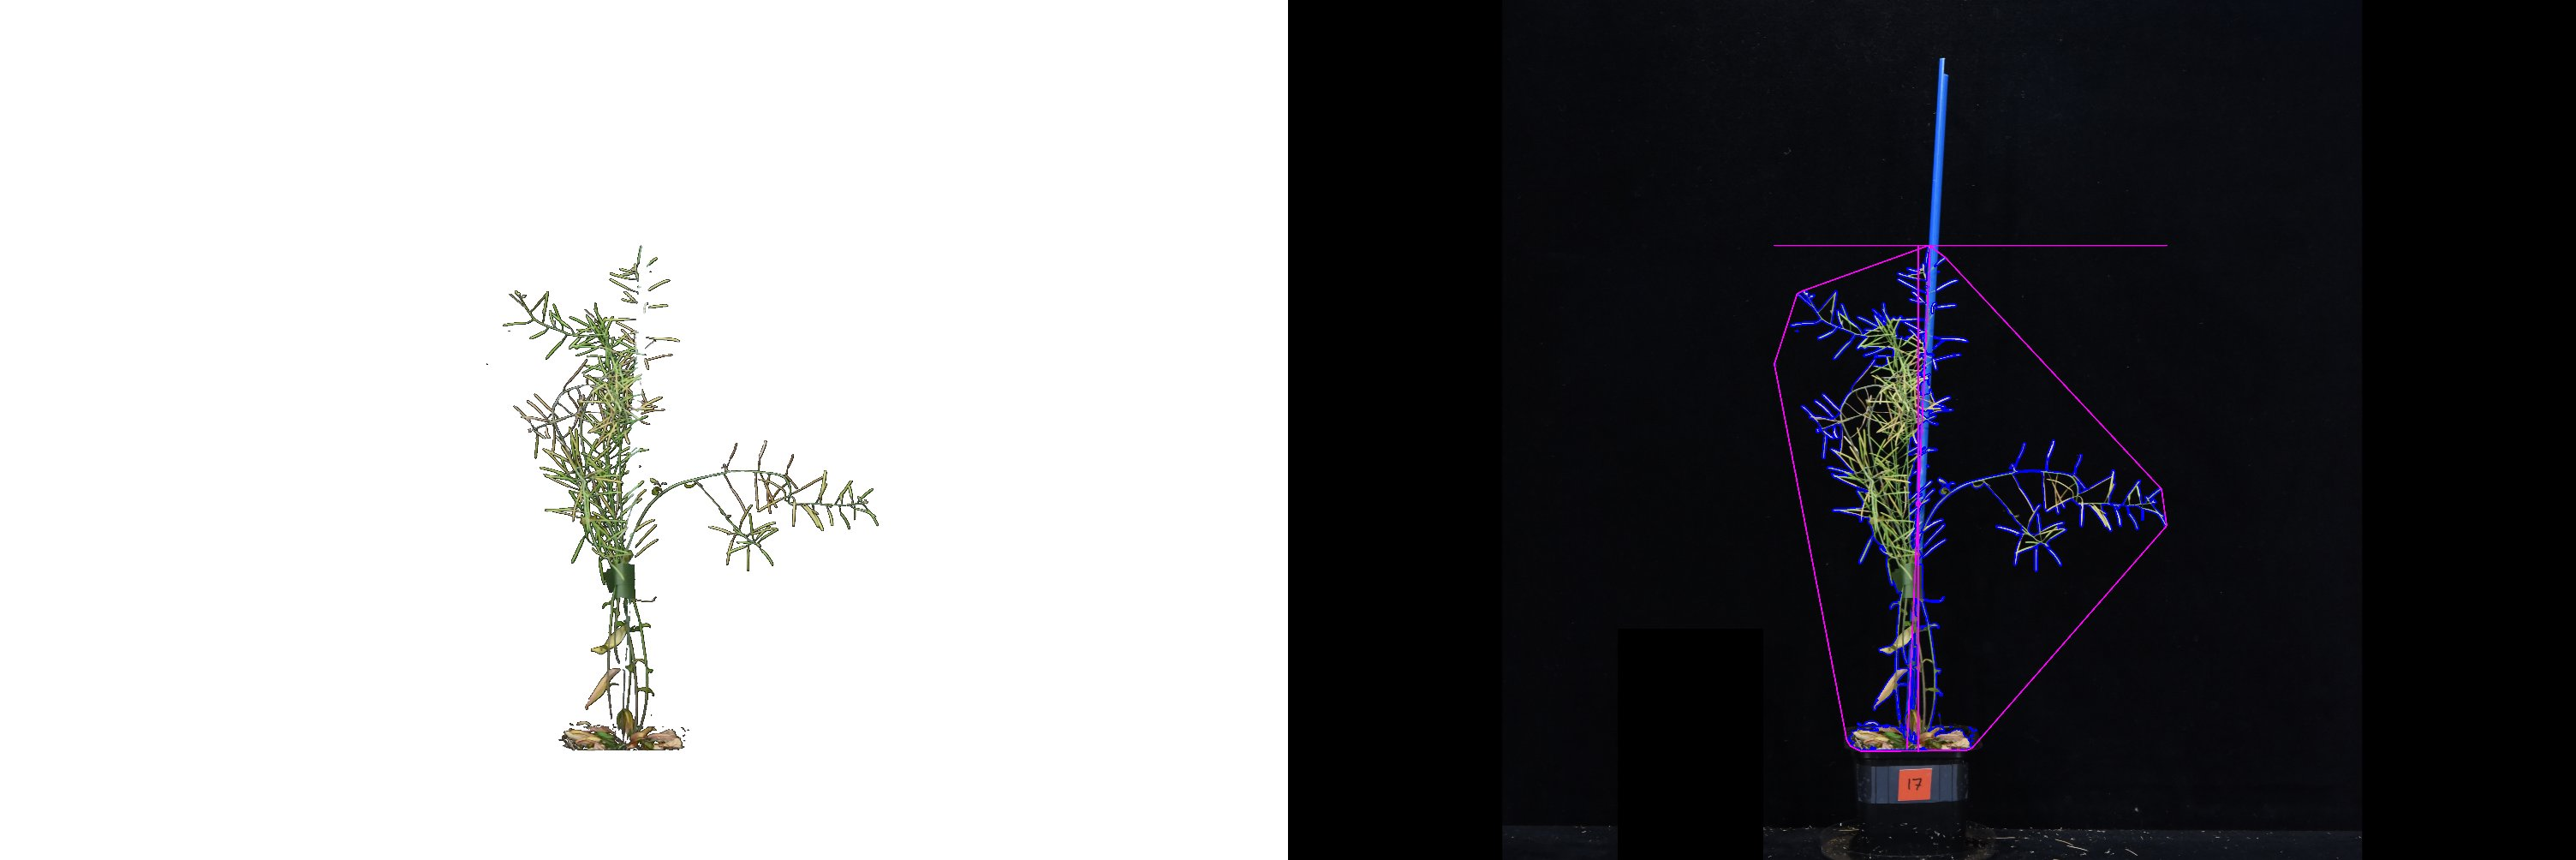
\includegraphics[width=0.95\linewidth]{inflorescence}
	\caption[Successfully analysed inflorescence.]{Successful segmentation of an inflorescence stem. In the right image, the convex hull of the plant is delineated in purple and the plant outline in blue.}
	\label{fig:inflorescence}
\end{figure}

\paragraph*{Final touches} As with the pipeline for the rosette growth, it is important to test your adjustments with multiple images. Especially test images of older plants, because senescence changes the overall colour of the plants quite dramatically.

\subsection{Batch analysis of multiple files}

Once you've checked that the pipelines work well for your images, it is time to batch process the whole folder. For this, we move from JupyterLab to the terminal. The important files now are \texttt{tray\_vis.py}/\texttt{plantcv\_vis.py} (containing the analysis pipeline) and \texttt{parallel\_trays.sh}/\texttt{parallel\_plants.sh} (containing the information for the batch processing, source folder, destination folder \textit{etc.}). 

\subsubsection{Adjust the pipeline file}

First we need to copy over any changes you made to the pipeline in JupyterLab in section \ref{opt} to the \texttt{.py} files. Unless you made comprehensive structural changes to the pipeline, the easiest way to do this is to manually adjust the values in the \texttt{.py} files accordingly (\textit{i.e.} if you changed a threshold value from 100 to 110 in the \texttt{.ipynb} file, you make the same change in the \texttt{.py} file).

\subsubsection{Adjust the batch file}

Next we need to adjust the \texttt{.sh} files. The lines you need to check are:

\begin{itemize}
	\item the first uncommented line: change the path so it points to the \texttt{plantcv-workflow.py} file in the plantcv conda environment of the used computer
	\item \texttt{-d}: change the path to point to your folder of images to be analysed 
	\item \texttt{-i}: change the path to point to your desired output folder
	\item \texttt{-p}: change the path to point to the correct pipeline (\texttt{.py}) file
\end{itemize}

\subsubsection{Run the batch analysis}

Now everything that remains is to run the batch analysis. Simply open a terminal in the folder containing the batch (\texttt{.sh}) file, check that you are in the correct conda environment and execute the batch file (example for the tray analysis):

\begin{bashcode}
	conda activate plantcv # make sure you are in the correct conda environment
	bash parallel_trays.sh # execute batch file
\end{bashcode}

\subsection{Data analysis}

\end{document}
